\documentclass{scrreprt}

% Texte
\usepackage[utf8]{inputenc}
\usepackage[T1]{fontenc}
\usepackage[french]{babel}
\usepackage[babel=true]{csquotes}
\usepackage{lmodern}
\usepackage{color}
\usepackage{minted}
\usepackage{caption}
\usemintedstyle{trac}

%%%%%%%%%%%%%%%%%%%%%
\usepackage{url}
\usepackage[top=2.1cm,bottom=2.2cm,left=2cm,right=2cm]{geometry}
\usepackage[final]{pdfpages}
%%%%%%%%%%%%%%%%%%%%%%%%%%%

%%%%%%%%%%% Pour sommaire cliquable %%%%%%%%%%
\usepackage{hyperref} % Créer des liens et des signets
\hypersetup{
	colorlinks=true, %colorise les liens
	breaklinks=true, %permet le retour à la ligne dans les liens trop longs
	urlcolor=blue, %couleur des hyperliens
	linkcolor=black, %couleur des liens internes
	citecolor=black,  %couleur des références
}
%%%%%%%%%%%%%%%%%%%%%%%%%%%%%%%%%%%%%%%%%%%%

% Images
\usepackage{float}
\usepackage{wrapfig}
\usepackage{graphicx}

% Couverture
\usepackage{templateINSA}
\initINSA

\title{Application de recettes}
\renewcommand\infoSmall{ASI4 2014-2015}
\author{Antoine \bsc{Augusti}\\ Thibaud \bsc{Dauce}}

\renewcommand\soustitre{Utilisation de BDD NoSQL}
\renewcommand\infoBig{PAO NoSQL}

\newcommand{\serviceProvider}{\texttt{Service Provider}}
\newcommand{\servicesProvider}{\texttt{Services Provider}}
\newcommand{\ioc}{\textit{IoC Container}}
\newcommand{\repositoryPattern}{\textit{Repository Pattern}}
\newenvironment{code}{\captionsetup{type=listing}}{}

%% -- Document
\begin{document}
	% titleINSA : Page de garde
	% #1 : descendre le titre du milieu (en mm)
	% #2 : lien de l'image de fond
	% #3 : décalage sur X de l'image de fond (en mm)
	% #4 : décalage sur Y de l'image de fond (en mm)
	% #5 : largeur de l'image de fond de #5 (en mm)
	% #6 : Crédit de l'image de fond
	\titleINSA{0}{images/fond.png}{0}{0}{225}{Licence CC - Wikimedia}
	\tableofcontents

	\chapter{Introduction}
		Dans la première partie de notre Projet d'Approfondissement et d'Ouverture, nous avons étudié les différents types de bases de données NoSQL au travers d'un état de l'art. Ce document, disponible sur Github à l'adresse \url{https://github.com/AntoineAugusti/NoSQL-etatart/tree/master/livrables/rapport}, avait pour objectif de montrer les avantages et les inconvénients d'un maximum de bases de données différentes afin d'obtenir une vision globale de l'écosystème NoSQL aujourd'hui. Malgré les exemples utilisés pour illustrer les propos tenus, ce document garde une approche très théorique.\\

Suivant naturellement notre premier état de l'art, l'objectif de ce deuxième document porte sur la mise en pratique des bases de données NoSQL dans un projet réel. Pour cela, nous nous sommes appuyés sur le projet de base de données des étudiants ASI de 3ème année. Le sujet de cette année était la réalisation d'une application de gestion de recettes de cuisine ainsi que d'invitation à des événements culinaires (l'énoncé est disponible en annexe \ref{cha:enonce_du_projet_de_base_de_donnees}). Les contraintes techniques des étudiants de 3ème année était la réalisation d'un client en C communiquant avec PostgreSQL, une base de données relationnelle. Nous avons trouvé intéressant de travailler sur le même sujet afin de pouvoir leur fournir une vision différente de la conception et de la modélisation d'une architecture de stockage de données en fonction du choix entre relationnel ou NoSQL.\\

Ce document est donc premièrement un rapport sur la modélisation et la conception de notre application, mais aussi un outil de travail pour les étudiants souhaitant approfondir leurs connaissances dans le domaine après notre intervention en cours de base de données\footnote{Voir notre intervention auprès des étudiants ASI de 3ème année sur YouTube : \url{https://www.youtube.com/watch?v=oIpjcqHyx2M}}.\\

Nous allons tout d'abord parler de Laravel, le framework web PHP retenu pour réaliser l'application, puis dans une deuxième partie, les choix effectués au niveau des bases de données NoSQL : les différents types de bases utilisés ainsi que les différentes modélisations possibles et retenues.

	\chapter{Utilisation du framework Laravel}
		Comme énoncé dans la première partie, nous avons fait le choix d'utiliser un framework nommé Laravel. Ce framework est assez récent et a pour objectif de faciliter le développement. Son slogan est \enquote{\textit{PHP that doesn't hurt. Code happy and enjoy the fresh air."}}. Depuis l'année 2013 Laravel a connu un succès important et il est depuis peu le framework PHP attirant le plus de recherches comme montré dans la figure \ref{fig:trends-php-frameworks}.

\begin{figure}[H]
	\centering
	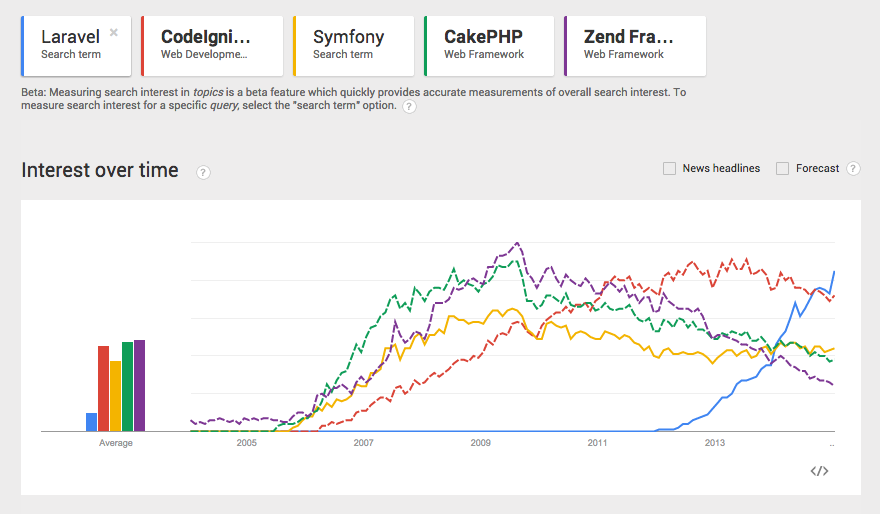
\includegraphics[width=1\textwidth]{images/trends-php-frameworks.png}
	\caption{Recherches Google pour les principaux frameworks PHP.}
	\label{fig:trends-php-frameworks}
\end{figure}

\section{Un framework MVC}
	Laravel est un framework mettant en avant une séparation très importante des modèles, des vues et des contrôleurs. Toutes les classes que nous avons créé se trouvent dans le dossier \verb|app/Insa| et sous l'espace de nom (\textit{namespace}) \verb|Insa|.\\

	Nous avons choisi une architecture modulaire organisée selon les entités. Dans chaque entité, on peut retrouver les dossiers suivants :
	\begin{itemize}
		\item \verb|Controllers| : les contrôleurs associés à l'entité ;
		\item \verb|Models| : les modèles associés à l'entité. Généralement il n'y a qu'une classe dans ce dossier qui correspond au singulier de l'entité, par exemple \verb|\Insa\Recipes\Models\Recipe| ;
		\item \verb|Presenters| : les classes qui ont pour objectif d'effectuer les transformations nécessaires afin de présenter les données brutes dans l'application web ;
		\item \verb|Repositories| : les classes d'accès aux bases de données ;
		\item \verb|Validation| : les classes comportant les règles de validation des entités.
	\end{itemize}

\section{Les \textit{Services Provider}}
	Les \verb|Services Provider| de Laravel sont de simples objets fournissant de la configuration pour l'application. Ils sont définis dans le fichier \verb|app/config/app.php|.\\

	Dans notre cas, nous avons créé un simple Service Provider \verb|LeoCardServiceProvider| qui effectue le lien de l'interface vers l'implémentation dans sa méthode \verb|register|.
	\begin{minted}{php}
	<?php
	public function register()
	{
		$this->app->bind('UserRepository', 'DatabaseUserRepository');
	}
	\end{minted}

\section{L'injection de dépendance}
	Nous n'instançons jamais notre contrôleur, Laravel s'en charge à notre place lorsque la route enregistrée est demandée. Pour instancier une classe, Laravel utilise un outil très puissant de résolution de dépendance grâce à l'introspection de PHP. Avant de créer l'objet nécessaire, elle détermine les classes requises par le constructeur.\\

	Si le constructeur nécessite un objet \verb|DatabaseUserRepository| comme dans notre cas, Laravel va l'instancier et le fournir au constructeur du contrôleur \verb|UsersController|.
	\begin{minted}{php}
	<?php
	public function __construct(DatabaseUserRepository $userRepository)
	{
	$this->userRepository = $userRepository;
	}
	\end{minted}

	De cette manière, nous avons accès au répertoire dans notre contrôleur sans effort.

\section{"Code to an interface"}
	La méthode présentée dans le paragraphe précédent présente l'avantage d'être simple à implémenter mais présente aussi un gros défaut : notre contrôleur est toujours lié à l'ORM via l'objet \verb|DatabaseUserRepository|.\\

	En réalité, notre contrôleur n'a pas besoin de savoir quel type de répertoire il utilise, l'unique besoin est une fonction appelée \verb|getBySerialBatch| prenant en paramètre un tableau d'identifiants NFC et retournant une collection d'utilisateurs. Ce qui est décrit ici est le principe même d'une interface. Nous avons donc créé une interface appelée \verb|UserRepository| et fournissant la signature de méthode requise. Bien évidement, notre répertoire \verb|DatabaseUserRepository| doit maintenant implémenter cette interface.\\

	Nous pouvons donc changer le pré-requis du constructeur de notre contrôleur par l'interface \verb|UserRepository|.
	\begin{minted}{php}
	<?php
	public function __construct(UserRepository $userRepository)
	{
	$this->userRepository = $userRepository;
	}
	\end{minted}

	Mais que va donc faire Laravel lorsqu'il va rencontrer l'interface. En effet, si le framework cherche à résoudre la dépendance, il va se heurter au problème qu'il est impossible d'instancier une interface. Nous avons donc besoin de définir un lien entre notre interface et notre implémentation.

\section{Utilisation d'un répertoire}

	\subsection{Pourquoi utiliser un répertoire}
		Dans le cas d'une application simple comme la notre, il aurait été parfaitement correct d'appeler les méthodes de l'ORM directement dans le contrôleur comme simplifié ci-dessous :
		\begin{minted}{php}
		<?php
		public function batch()
		{
		return User::whereIn('serial', Input::get('data'));
		}
		\end{minted}

		Mais dans le cas d'une application plus complexe, il est préférable de dissocier ses contrôleurs de l'ORM afin d'améliorer la maintenabilité de l'application et de permettre l'utilisation d'un autre système de stockage.

	\subsection{Utilisation d'un répertoire dans notre projet}
		Afin de montrer les possibilités du framework Laravel ainsi que de permettre aux futurs étudiants allant travailler sur l'application de partir sur de bonnes bases, nous avons décidé d'implémenter un répertoire pour les utilisateurs.\\

		Ce répertoire se présente sous la forme d'une classe nommée \verb|DatabaseUserRepository| proposant une seule méthode : \verb|getBySerialBatch|. Cette méthode prend en paramètre un tableau contenant les différents numéros de carte NFC et retourne une collection d'objets \verb|User| via la méthode \verb|whereIn| de l'ORM Eloquent.\\

		Maintenant, afin de découpler nos contrôleurs de l'ORM, nous devons utiliser notre répertoire. Pour cela, Laravel nous propose deux solutions :
		\begin{itemize}
			\item Instancier l'objet normalement dans la méthode ;
			\item Utiliser l'outil d'injection de dépendance de Laravel.
		\end{itemize}

\section{Routes}
	Dans la partie précédente, nous avons les différentes routes nécessaire à la mise en place d'un CRUD. Laravel implémente cela facilement via une façade nommée tout simplement \verb|Route|.

	\begin{minted}{php}
	<?php
	Route::get('users/batch', 'UsersController@batch');
	\end{minted}
	Notre application contient une seule route dans le fichier \verb|app/route.php|, définie comme ci-dessus.\\

	Tout d'abord, nous appelons la méthode \verb|get| parce que dans une optique CRUD, nous cherchons à obtenir des informations. Cette méthode prend en premier paramètre l'URI associé à la route et en deuxième paramètre une chaîne de caractère  formatée comme \verb|ControllerObject@method|. Dans notre cas, lorsque l'utilisateur fait une requête GET sur l'URI \verb|users/batch|, Laravel va appeler la méthode \verb|batch| sur l'objet \verb|UsersController|.

	\subsection{Qu'est-ce qu'une façade}
		Une façade est un classe spécifique qui permet d'appeler des méthodes publiques d'une instance d'un objet via des appels statiques sur la façade.\\

		Par exemple, lorsque j'appelle une méthode statique sur la façade \verb|Route|, Laravel va en réalité appeler une méthode publique d'une instance d'une classe appelée \verb|Illuminate\Routing\Router| stockée dans l'application.\\

		Vous pouvez en savoir plus sur les façades Laravel dans la documentation \url{http://laravel.com/docs/facades}

\section{Le modèle}
	Laravel utilise son propre ORM appelé Eloquent. Ce dernier nécessite la création d'une classe par ressource de l'application. Notre application a donc un modèle nommé \verb|User| situé dans le répertoire \verb|app/models|. Ce dernier hérite du modèle Eloquent qui fournit toutes les méthodes d'accès à la base de données telles que \verb|where|, \verb|find|, \verb|save|...\\

	Dans notre modèle, nous devons définir plusieurs attributs :
	\begin{itemize}
		\item \verb|$table| : cet attribut permet de définir la table associée au modèle. Même si Eloquent est assez intelligent pour définir le pluriel du nom de l'objet (User => users), pour des raisons de lisibilité, nous l'avons redéfini.
		\item \verb|$fillable| : afin de répondre au problème de \verb|MassAssigment|, Eloquent demande de fournir un tableau contenant les attributs du modèle qu'il sera possible de sauvegarder directement via la méthode \verb|create| afin d'éviter qu'un utilisateur mal intentionné insère dans la base de données des champs non voulus. (plus d'informations sur \url{http://laravel.com/docs/eloquent#mass-assignment})
	\end{itemize}

\section{Les contrôleurs}
	Toujours dans une optique CRUD, Laravel nous encourage à créer un contrôleur pour chaque ressource. Notre application ne contient qu'une seule ressource pour le moment appelée \verb|User|, notre contrôleur (par convention) aura donc le nom de \verb|UsersController| et sera situé dans le répertoire \verb|app/controllers|.\\

	Cet objet aura une seule méthode, la méthode \verb|batch| définie dans les routes comme la méthode à appeler.

\section{Conclusion}
	Cette approche par répertoire et par interface nous a permis de créer une application très solide et sans grande dépendance. Par exemple, si nous souhaitons changer d'implémentation, remplacer par exemple la base de données par un système de fichier, il suffit de définir un nouveau répertoire \verb|FileUserRepository| implémentant l'interface \verb|UserRepository| et de compléter les méthodes nécessaires. Ensuite, en changeant le lien dans le Service Provider nous obtenons une nouvelle implémentation sans jamais avoir à ouvrir nos contrôleurs ce qui aurait pu être une source de bugs lors du changement.\\

	La principale limitation de ce système provient du langage PHP, qui ne permet pas de spécifier des types de retour. La nouvelle implémentation doit donc se référer à la documentation et suivre à la lettre les instructions de retour spécifiées dans l'interface même si ces dernières ne sont pas obligatoire au niveau du langage. Ce problème peut être contourné via l'utilisation de la machine virtuelle \verb|HHVM| de Facebook et du langage \verb|Hack|, compatible avec PHP et introduisant un typage statique.

	\chapter{Modélisation NoSQL}
		\section{MongoDB} % (fold)
\label{sec:mongodb}

	\subsection{Intégration avec PHP et Laravel}% (fold)
	\label{sub:integration_avec_php_et_laravel}

		MongoDB bénéficie d'une extension PHP facilement installable via PEAR (le gestionnaire d'extensions de PHP). Deux limitations existent néanmoins : le support de la version 3.0 de MongoDB n'est pas encore pris en charge et l'extension n'est pas encore compatible avec la toute dernière version majeure de PHP (PHP 7.0) prévue pour fin novembre. La mise à jour de l'extension vers la toute dernière version de MongoDB et de PHP sera sans doute effective rapidement.\\

		Afin de faciliter le développement, il a été décidé d'utiliser un ORM. Dans le cas des bases de données orientées documents, on parle alors d'un ODM pour \textit{Object Document Mapping}. Par simplification, on peut dire qu'un ODM n'est ni plus ni moins qu'un ORM pour une base de données orientée documents. Plusieurs grands ORM existent dans le monde des frameworks PHP : Doctrine et Eloquent sont deux des plus connus. Tous deux proposent un ODM associé. Doctrine présente l'avantage de permettre une intégration de MongoDB via un package PHP officiel\footnote{Les bases de données peuvent être intégrées à l'aide d'un package PHP, écrit en C et qui doit être rajouté à la configuration de PHP ou d'un simple client vers la base de données. Dans le second cas, le client est écrit en PHP et les performances sont moins bonnes.}. Eloquent supporte le système de base de données MongoDB via un package non-officiel (développé par jenssegers) appelé tout simplement \verb|mongodb|. Dans les deux cas, l'outil permet de gérer toutes les opérations de base ainsi que les documents imbriqués. Nous avons décidé d'utiliser Laravel et donc son ORM officiel Eloquent, nous allons donc utiliser le package \verb|jenssegers/mongodb| dans sa version 2.0.\\

		L'utilisation d'une base de données NoSQL est souvent délicate car il en existe de nombreux types différents et les intégrations ne sont donc pas forcément toutes développées (et rarement intégrée par des packages officiels). Il est donc préférable de se limiter aux bases de données les plus utilisées pour chaque type (MongoDB pour les bases de données orientées documents, Redis pour les bases de données orientées clé / valeur par exemple.). Dans notre cas, MongoDB étant très utilisée, il existe donc de nombreuses intégrations, comme nous l'avons vu pour PHP, mais aussi pour les différents ORM du marché ainsi que pour la plupart des solutions de test de l'écosystème (nous ne détaillerons pas les solutions de test dans ce rapport).

	% subsection integration_avec_php_et_laravel (end)

% section mongodb (end)

\section{Modélisation de la base de données orientée documents}% (fold)
\label{sec:modelisation}

	Comme expliqué dans notre état de l'art des bases de données NoSQL\footnote{Voir notre état de l'art sur les bases de données NoSQL : \url{https://github.com/AntoineAugusti/NoSQL-etatart/tree/master/livrables/rapport}}, il n'existe pas de schéma fixe pour ces dernières. Pour autant, lors du développement d'une véritable application, il est nécessaire pour les développeurs de se fixer des schémas afin de pouvoir utiliser la base de données.\\

	Nous avons organisé notre base de données en 4 collections : \verb|recipes|, \verb|locations|, \verb|guests| et \verb|events|.

	\subsection{Diagramme de stockage}

		\begin{figure}[H]
			\centering
			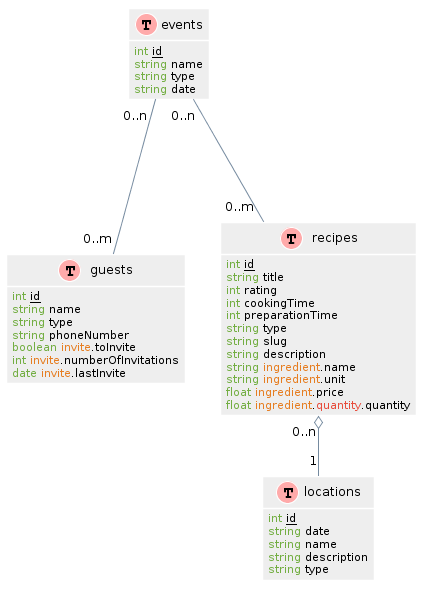
\includegraphics[width=0.5\textwidth]{images/diagramme-stockage.png}
			\caption{Diagramme de stockage de l'application dans une base de données orientée documents.}
			\label{fig:diagramme-stockage}
		\end{figure}

		Le diagramme de stockage de notre application est présenté dans la figure~\ref{fig:diagramme-stockage}. Les clés primaires de chaque collection sont soulignées. Les documents imbriqués sont représentés par des variations de couleurs dans les champs d'une collection. Les champs supplémentaires nécessaires aux relations \texttt{m..n} ne sont pas représentés.

	\subsection{Recettes et ingrédients}

		Les recettes sont stockées dans la collection \verb|recipes|. Il n'existe pas de collection pour les ingrédients et leur quantité associée car nous avons décidé d'utiliser l'imbrication de documents afin de les stocker directement dans chaque recette.

		\paragraph{Avantage de la solution}% (fold)
			Lors de la récupération de chaque recette, les ingrédients sont automatiquement récupérés. Nous savons que dans la majorité des cas les informations sur les ingrédients seront nécessaire à l'affichage d'une recette, cette solution présente donc un avantage au niveau des performances (un seul document est à récupérer pour afficher une recette avec ses ingrédients). De plus, dans le cas présent, les ingrédients sont très succints (nom, unité, quantité et prix) et chaque recette ne possède que peu d'ingrédients donc cette solution ne va pas surcharger notre document parent.
		% paragraph avantage_de_la_solution (end)

		\paragraph{Désavantage de la solution}% (fold)
		\label{par:desavantage_de_la_solution}
			Avec cette approche, il est très coûteux de récupérer la liste de tous les ingrédients car il faut parcourir toutes les recettes. De plus, cette solution nous oblige à dupliquer des informations pour chaque recette ayant des ingrédients identiques. Mettre à jour un ingrédient spécifique nous obligera à modifier indépendamment chaque recette utilisant cet ingrédient.
		% paragraph desavantage_de_la_solution (end)

		\paragraph{Avantages contre désavantages}% (fold)
			Dans notre application, le cas d'utilisation le plus utilisé sera l'affichage de recette. Il est donc préférable d'optimiser les lectures via l'imbrication. La possibilité de mettre à jour les ingrédients n'est pas prévue et dans le cas où elle serait ajoutée, elle resterait très rare par rapport à l'affichage. Le coût de mise à jour n'est donc pas un problème.
		% paragraph avantages_contre_desavantages (end)

	\subsection{Localisations}

		Les localisations sont stockées dans la collection \verb|locations|. Pour les localisations, trois choix sont possibles : stocker les localisations directement dans les documents \verb|recipe|, stocker les recettes dans les documents \verb|location| ou encore sotcker les documents \verb|recipe| et \verb|location| de manière indépendante et les lier via une clé étrangère.

		\paragraph{Avantage du stockage dans le document recipe}% (fold)
			Cette méthode de stockage permet d'améliorer les performances lors de l'affichage d'une recette. Cas d'utilisation très courant.
		% paragraph avantage_de_la_solution (end)

		\paragraph{Désavantage du stockage dans le document recipe}% (fold)
			Cette méthode complexifie le traitement des recettes via leur localisations. Il est plus coûteux d'afficher toutes les recettes d'une localisation par exemple.
		% paragraph desavantage_de_la_solution (end)

		\paragraph{Avantage du stockage dans le document location}% (fold)
			Cette méthode de stockage permet d'améliorer les performances lors de l'affichage d'une localisation avec toutes ses recettes.
		% paragraph avantage_de_la_solution (end)

		\paragraph{Désavantage du stockage dans le document location}% (fold)
			Les documents \verb|location| peuvent devenir très importants (très grande taille) si de nombreuses recettes sont stockées au même endroit.
		% paragraph desavantage_de_la_solution (end)

		\paragraph{Avantage du stockage séparé}% (fold)
			Cette méthode permet de gérer les recettes et les localisations de manière indépendante. Cette méthode est aussi la plus simple au niveau de la modélisation.
		% paragraph avantage_de_la_solution (end)

		\paragraph{Désavantage du stockage séparé}% (fold)
			Les requêtes ne sont pas optimisées dans les deux cas car MongoDB doit effectuer deux requêtes pour afficher une recette et $(n+1)$ requêtes pour afficher une localisation avec ses recettes.
		% paragraph desavantage_de_la_solution (end)

		\paragraph{Conclusion}% (fold)
			Nous avons décidé de gérer les recettes et les localisations de manière indépendante afin de simplifier la modélisation. Cette solution n'est pas parfaite et il faudrait savoir si il est préférable d'améliorer l'affichage des recettes ou celle des localisations ainsi que le nombre de recettes maximal pour une localisation (afin de savoir la taille probable de nos documents \verb|location|). Ce problème illustre les difficultés de modéliser une base de données lorsque les cas d'usages ne sont pas parfaitement connus.
		% paragraph conclusion (end)

		\paragraph{Solution alternative}% (fold)
			Il est également possible de combiner les deux stockages en dupliquant les informations. Par exemple, stocker dans le document \verb|recipe| sa localisation et stocker dans les documents \verb|location| un sous-ensemble (la recette sans ses ingrédients par exemple) de recette afin de limiter la taille. Cette solution présente les avantages des deux types de stockages et évite les requêtes multiples au détriment de la simplicité de la modélisation et des mises à jour des documents.
		% paragraph solution_alternative (end)

	\subsection{Invités}

		Les invités sont stockées dans la collection \verb|guests|. Cette collection est très simple car elle ne stocke qu'une seule entité. L'utilisation de MongoDB dans ce cas est la même que pour une base de données relationnelle.

	\subsection{Évènements}

		Les évènements sont stockées dans la collection \verb|events|. Tout comme pour les invités, cette collection est très simple car elle ne stocke qu'une seule entité.

	\subsection{Relations \texttt{m..n}}

		Il existe entre les invités et les évènements et entre les recette et les évènements des relations \texttt{m..n}. En relationnel, ces relations sont gérées par une table de pivot contenant deux clés étrangères avec les identifiants de chaque modèle et optionnellement des caractéristiques de la relation. Les table pivots ne sont pas du tout optimisées pour les bases de données orientées documents. En effet, avec ces dernières, il est nécessaire d'effectuer une requête supplémentaire afin de récupérer le document correspondant à la relation. Toujours dans l'optique d'optimiser les lectures, notre ODM nous propose de gérer les relations \texttt{m..n} grâce à un tableau d'identifiants à la place d'une collection pivot. Il existe donc dans le document \verb|event| par exemple, deux tableaux d'identifiants : \verb|guest_ids| et \verb|recipe_ids|. Ces tableaux sont répétés dans le document \verb|guest| et dans le document \verb|recipe| avec un tableau \verb|event_ids|.

		\paragraph{Avantage de la solution}% (fold)
			À partir du moment où le document \verb|event| est récupéré, il est possible d'effectuer directement une nouvelle requête afin de récupérer les recettes ou les invités associés sans passer par une requête supplémentaire sur une collection pivot.
		% paragraph avantage_de_la_solution (end)

		\paragraph{Désavantage de la solution}% (fold)
			L'ajout ou la suppression d'une relation entre deux documents passent par la mise à jour des deux documents et non pas par l'insertion ou la suppression d'un document pivot unique.
		% paragraph desavantage_de_la_solution (end)

		\paragraph{Conclusion} % (fold)
			Le cas d'utilisation le plus courant de l'application sera la lecture des recettes. Il est donc nécessaire d'optimiser les requêtes en lecture, même si ces optimisations se font au détriment des requête en écriture (cas d'utilisation beaucoup plus rare). La solution de suppression de la table pivot est donc plus performante pour nos cas d'utilisation.
		% paragraph conclusion (end)

	\subsection{La vue AInviter}

		Dans le cadre du projet de base de données, il a été demandé de faciliter l'accès aux personnes à inviter en créant une vue des invités avec si oui ou non ils ont déjà été invités, le nombre d’événements auxquels ils ont participé et la date de la dernière invitation si cette dernière a eu lieu.\\

		Le système de vue n'existant pas dans les bases de données orientées document, cette optimisation passe par un nouveau document dupliqué (un booléen indiquant si la personne a déjà été invitée, le nombre d'invitations reçues par cette personne et la date de la dernière invitation) et imbriqué dans les invités afin de stocker ces informations. Ce stockage sous forme de document imbriqué va améliorer les performances de lecture mais détériorer les performances en écriture. En effet, à chaque nouvelle invitation d'un invité, il est nécessaire de mettre à jour ce document imbriqué avec les nouvelles valeurs. La duplication des informations n'est pas une mauvaise chose car l'application a des besoins beaucoup plus importants en lecture qu'en écriture.

% section modelisation (end)

\section{Utilisation d'une base de données clé-valeur}
	\subsection{Le besoin d'utiliser une base de données clé-valeur }
		Nous avons vu dans la sous-section précédente \ref{par:desavantage_de_la_solution} qu'il était très coûteux de récupérer la liste de tous les ingrédients. Pourtant cette opération doit être effectuée lors de l'ajout d'une recette. En effet, lors de l'ajout de la recette, il est nécessaire de choisir quels ingrédients sont nécessaires à la réalisation de la recette.\\

		Pour aider l'utilisateur, il est utile de lui suggérer les ingrédients déjà connus de l'application, lorsque celui-ci ajoute les ingrédients nécessaires à sa nouvelle recette. Il apparaît comme inenvisageable de devoir parcourir toutes les recettes, extraire tous les ingrédients de chaque recette et construire une liste d'ingrédients sans duplicatas pour répondre à ce cas d'utilisation.\\

		C'est lors de problématiques comme celles-ci qu'une base de données clé-valeur est utile. Une base de données clé-valeur peut permettre de stocker une valeur, issue d'un calcul coûteux, pendant une courte période. Par exemple, imaginons que l'on souhaite proposer un \enquote{classement} d'utilisateurs d'un jeu. Ce classement sera établi en fonction de leurs actions dans le jeu, de leurs réponses sur le forum, de leur activité\dots{} L'établissement de ce classement est très coûteux en terme de temps de calcul pour une base de données, pourtant le besoin d'un classement est bien réel. Il n'est pas envisageable de faire le calcul nécessaire à l'établissement du classement dès qu'un utilisateur cherche à consulter celui-ci. On pourrait donc envisager de mettre tout ou partie du résultat du calcul du classement dans une base de données clé-valeur, et rafraîchir ce résultat régulièrement, à l'aide d'une tâche CRON par exemple.

	\subsection{Stockage de la liste des ingrédients en base de données clé-valeur}
		\subsubsection{Problème rencontré}
			L'idée principale est d'avoir accès facilement à une liste de tous les ingrédients. En réfléchissant un petit peu plus longtemps, on se rend compte qu'il pourrait être utile d'avoir des informations supplémentaires comme le prix et l'unité de la quantité associée à l'ingrédient. Le problème est que le prix d'un ingrédient n'est pas toujours le même, et l'unité de la quantité associée à l'ingrédient peut varier selon les goûts de chacun.\\

		\subsubsection{Solution retenue}
			Pour autant, l'utilisateur appréciera de se voir proposer des valeurs par défaut cohérentes lorsque celui-ci ajoutera un ingrédient déjà connu de l'application à une recette créée. On décide alors de définir le prix de l'ingrédient comme la moyenne des prix indiqués pour le même ingrédient (utilisé dans les autres recettes) et de fixer l'unité de la quantité associée à l'ingrédient comme celle la plus souvent choisie par les utilisateurs.\\

			Lors de l'ajout d'un ingrédient à une recette, si cet ingrédient n'existait pas encore, l'ingrédient est rajouté à la liste des ingrédients en base de données clé-valeur, avec son prix et l'unité de la quantité choisie. Si l'ingrédient existait déjà, le prix est mis à jour en calculant une nouvelle moyenne et l'unité de la quantité associée reste inchangée. La clé a un temps d'expiration de 30 minutes, ce qui veut dire que la liste des ingrédients avec la moyenne des prix et les unités sera automatiquement régénérée 30 minutes après la création de la clé. On trouve ici un bon compromis : un accès quasi instantané à une information coûteuse à calculer et la garantie de la quasi cohérence de cette information.\\

			Au final on obtient un grand gain de performance au prix de quelques lignes de code à écrire en plus et d'une base de données clé-valeur légère à déployer.


	\pageQuatriemeCouverture{Département ASI}{02 32 95 97 79}{asi@insa-rouen.fr}
\end{document}